\documentclass{beamer}
\usepackage{ctex, hyperref}
\usepackage{calligra}
%\usepackage[colorlinks,linkcolor=black]{hyperref}
\usepackage[T1]{fontenc}
\author{杨秉学}
\title{毕业设计结题报告}
\subtitle{基于 Qume 模拟器移植 rCore 操作系统的开发与实现}
\institute{华北电力大学控制与计算机工程学院}
\date{\today}
\usepackage{Ncepu}

\begin{document}

\kaishu
\begin{frame}
	\titlepage
	\begin{figure}[htpb]
		\begin{center}
        
\includegraphics[width=0.2\linewidth]{pic/Ncepu_University_Logo.eps}
		\end{center}
	\end{figure}
\end{frame}
\begin{frame}
\tableofcontents[sectionstyle=show,subsectionstyle=show/shaded/hide,subsubsectionstyle=show/shaded/hide]
\end{frame}


\section{课题背景}

\begin{frame}{为什么要研究该项目?}
\begin{itemize}
\item 某国家的技术封锁
    \begin{figure}
        \centering
        
\includegraphics[height=0.6\textheight]{pic/trump_huawei.png}
        \caption{某国家元首签署制裁令}
    \end{figure}
% \item 中文支持请选择 Xe\LaTeX{} 编译选项
%     \begin{figure}
%         \centering
%         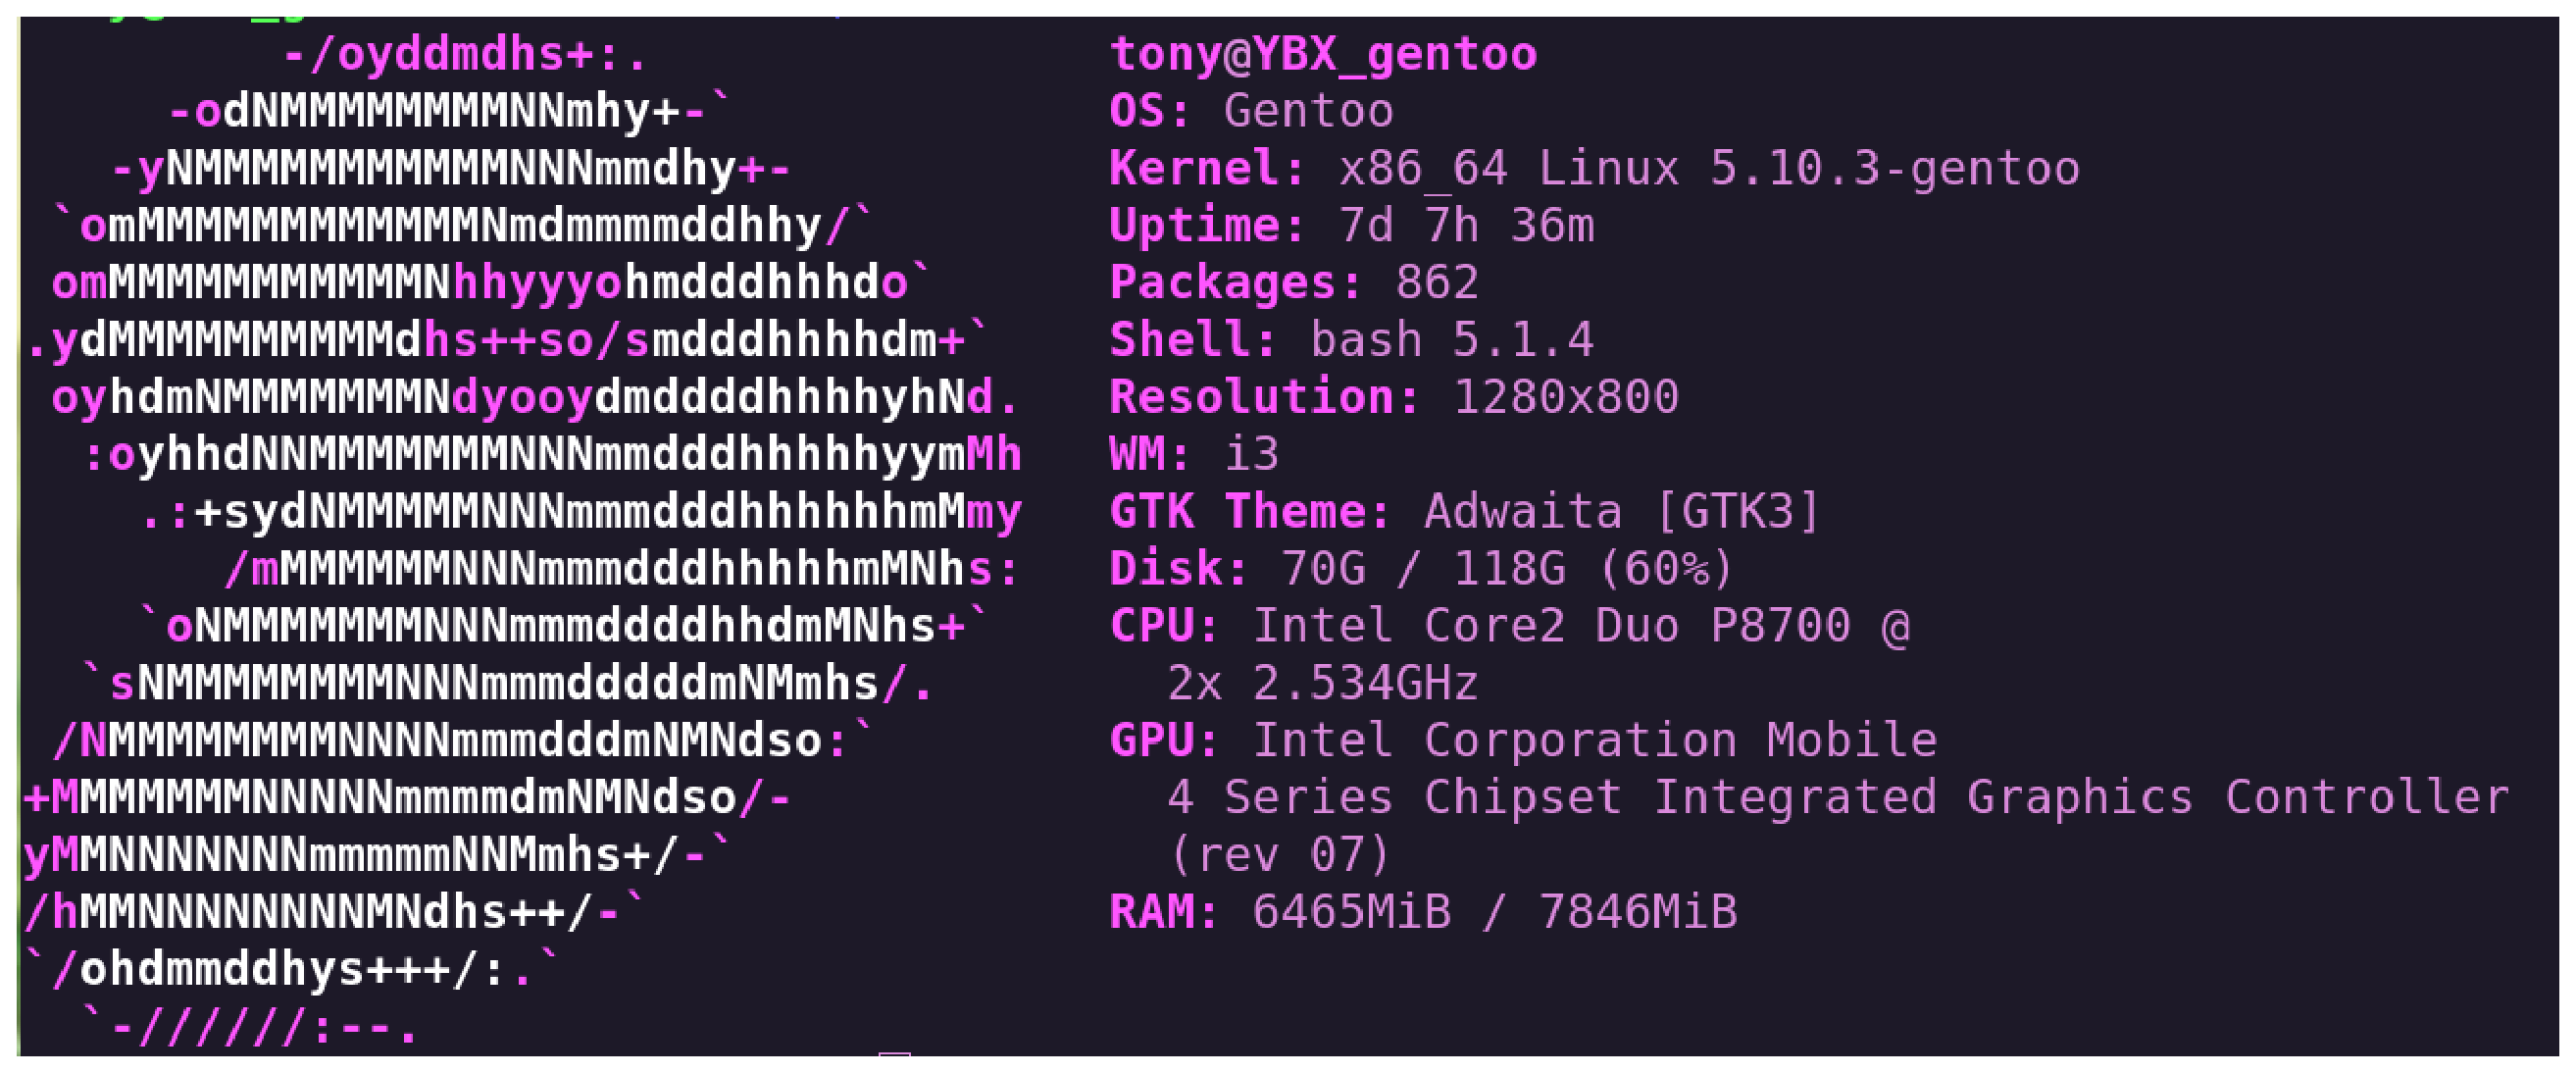
\includegraphics[height=0.4\textheight]{pic/gentoo_Logo.eps}
%         \caption{系统环境}
%     \end{figure}
\end{itemize}
\end{frame}

\section{研究现状}

\subsection{国外研究现状}

\begin{frame}{国外现状}
    \begin{figure}
        \centering
        
\includegraphics[height=0.6\textheight]{pic/SiFive.png}
        \caption{国外研究现状}
    \end{figure}
 
\end{frame}

\subsection{国内研究现状}

\begin{frame}{国内现状}
    \begin{figure}
        \centering
        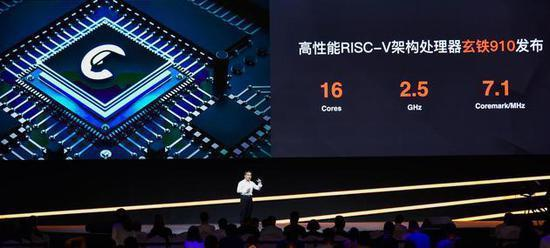
\includegraphics[height=0.6\textheight]{pic/阿里_Android.jpeg}
        \caption{国内研究现状}
    \end{figure}
 
\end{frame}

\section{研究内容}

\begin{frame}{毕设研究内容}
\begin{itemize}
\item 将Linux移植到RISC-V平台
\item 移植文件系统
\item 拥有简单的网络功能
\item 可以运行一个简单的程序
\end{itemize}
\end{frame}

\section{实验内容}
\begin{frame}
	\begin{itemize}
    \item 视频演示:https://www.bilibili.com/video/BV1QU4y1H7AE
    \begin{figure}
        \centering
        
\includegraphics[height=0.6\textheight]{pic/演示二维码.png}
        \caption{可以扫描一下二维码吗?}
    \end{figure}
	\end{itemize}
\end{frame}

\section{总结}
\begin{frame}{与前人比较}
    \begin{itemize}
       \item Linux、Qemu、GNU工具链等软件使用最新的完成了任务
       \item 解决了使用新版本软件时的一些列问题
    \end{itemize}
\end{frame}

% \section{参考文献}
% \begin{frame}[allowframebreaks]
% \bibliography{ref}
% \bibliographystyle{alpha}
% \end{frame}

\begin{frame}
\begin{center}
{\Huge\calligra Thanks!}
\end{center}
\end{frame}

\end{document}
